
针对式(\ref{eq:311t3}.c),结合附加的第二类边界条件,由无旋条件,
我们设$\v{u}=\nabla \phi$,则$\phi$满足Neumann边界条件的PDE:
\begin{equation}\label{eq:41t3}
\begin{cases}
\nabla ^2 \phi = & 0 \\
\frac{\partial \phi}{\partial \v{n}}|_{bn}= & v_{bn}(\v{x})-\v{v_E}\cdot \v{n}-\v{v_N}\cdot \v{n}\\
\end{cases}
\end{equation}
其中$\v{v_E},\v{v_N}$是(\ref{eq:311t3}.a),(\ref{eq:311t3}.b)的特解。
方程\eqref{eq:41t3}可以使用格林函数法求解\cite{GreenFunction},

\textbf{流体动力学积分型方程}

\textbf{质量体} 的边界是随时间变化的,而\textbf{控制体} 的边界是不变的。
\textbf{Reynolds 输运}定理是联系质量体和控制体的桥梁,可以把关于质量体的守恒定律轻松转化为关于控制体的守恒定律。
它的陈述为:某一质量体的某一物理量在某时刻的随体导数等于该时刻相同体积相同形状的控制体该物理量的局部导数与该物理量的通过
该控制体的表面输运量。

下面设物理量为$Q$,时刻为$t_0$, 用$D^*(t)$表示质量体,而用$D$表示$D^*(t_0)$,$\Sigma$表示$D$的边界曲面,$\v{v}$是流体速度场,$d\tau$表示体积微元。则有
\begin{equation}
\frac{D}{Dt}[\iiint\limits_{D^*(t)}Qd\tau]_{t=t_0}=\iiint\limits_{D}\frac{\partial Q}{\partial t} d\tau + \oiint\limits_{\Sigma} Q\v{v}\cdot\v{n}dA
\end{equation}

下面给出两种推导,
\begin{align*}
\frac{D}{Dt}[\iiint\limits_{D^*(t)}Q(\v{x},t)d\tau] = & \iiint\limits_{D^*(t)} \frac{D}{Dt}[Q(\v{x},t)d\tau] \\
= & \iiint\limits_{D^*(t)} [\frac{DQ}{Dt}d\tau+Q\frac{D(d\tau)}{Dt}] \\
= & \iiint\limits_{D^*(t)} [\frac{DQ}{Dt}+Q\nabla \cdot \v{v}]d\tau, \,\,\text{体膨胀率的定义}\\
= & \iiint\limits_{D^*(t)} [\frac{\partial Q}{\partial t} + \v{v} \cdot \nabla Q +Q \nabla \cdot \v{v} ] d\tau \\
= & \iiint\limits_{D} \frac{\partial Q}{\partial t}d\tau + \iiint\limits_{D^*(t)} \nabla\cdot(Q\v{v})d\tau\\
= & \iiint\limits_{D} \frac{\partial Q}{\partial t}d\tau + \oiint\limits_{\Sigma} Q\v{v}\cdot \v{n} dA, \,\,\text{Gauss 公式}
\end{align*}

另一个推导要结合图示和一些几何直观,如图\ref{fig:412}所示:

\begin{figure}[!ht]
\centering
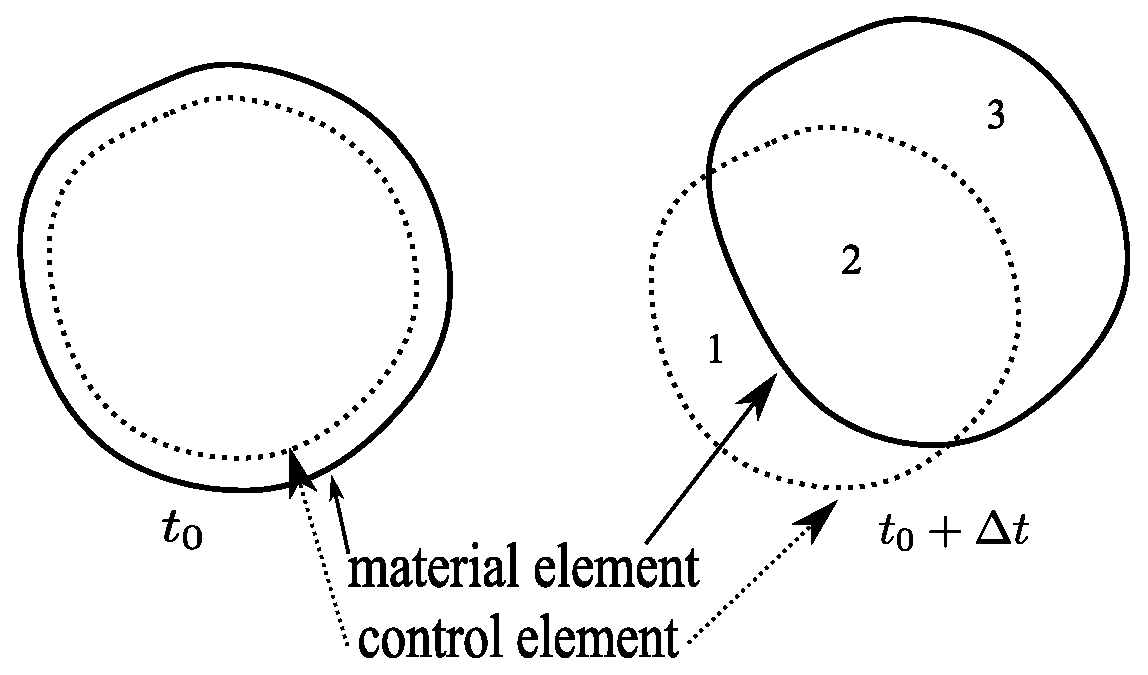
\includegraphics[width=5cm]{reynolds_derivation_illustration.eps}
\caption{雷诺输运方程推导图示}\label{fig:412}
\end{figure}
首先由随体导数的定义:
\begin{equation}
\frac{D}{Dt}[\iiint\limits_{D^*(t)}Qd\tau]_{t=t_0}=\lim_{\Delta t \to 0} \left[\frac{\iiint\limits_{D^*(t_0+\Delta t)}Q(\v{x},t_0+\Delta t) d\tau - \iiint\limits_{D^*(t_0)} Q(\v{x},t_0) d\tau  }{\Delta t}\right]
\end{equation}
积分区域$D^*(t_0+\Delta t)$可以写成$(1+2)+(3-1)$,数字所代表的区域如图\ref{fig:412}所示,注意到(1+2)仍表示控制体描述的区域,与$t_0$时刻相同,所以我们
进一步有:
\begin{align}\label{eq:41reynoldsD}
\frac{D}{Dt}[\iiint\limits_{D^*(t)}Qd\tau]_{t=t_0}=&\lim_{\Delta t \to 0} \left[
\frac{\iiint\limits_{D^*(t_0)}Q(\v{x},t_0+\Delta t) d\tau - \iiint\limits_{D^*(t_0)} Q(\v{x},t_0) d\tau  }{\Delta t}
\right]\nonumber\\
+&\lim_{\Delta t \to 0}\left[\frac{\iiint\limits_{D^*_3(t_0+\Delta t)}Q(\v{x},t_0+\Delta t) d\tau - \iiint\limits_{D^*_1(t_0+\Delta t)} Q(\v{x},t_0+\Delta t) d\tau  }{\Delta t}
\right]\nonumber\\
=& \iiint\limits_{D^*(t_0)}\frac{\partial Q}{\partial t} d\tau + \oiint\limits_{\Sigma} Q\v{v} \cdot \v{n} dA
\end{align}
式\eqref{eq:41reynoldsD}中第一项由于控制体的体积形状不变,所以对时间求导数可以挪到积分号里面;第二项根据问题的几何性质,
从1到3的体积变化由表面的流量引起,所以可以将体积的瞬时变化率转换为面积分的形式。

Reynolds 输运公式中取$Q$为不同的物理量,可以将Lagrange观点下的守恒方程(关于质量体)转化为Euler观点下的守恒方程(关于控制体)。

\textbf{质量守恒积分方程}:令$Q=$密度$\rho$,该守恒方程对任意坐标系均成立,对于质量体有:
\begin{equation}
\frac{D}{Dt} \iiint\limits_{D^*(t)}\rho d\tau =0
\end{equation}
应用Reynolds输运公式得到,对于控制体的质量守恒方程为
\begin{equation}\label{eq:41Conti}
\iiint\limits_{D}\frac{\partial \rho}{\partial t} d\tau = - \oiint\limits_{\Sigma} \rho \v{v}\cdot \v{n} dA
\end{equation}
即控制体内质量的变化等于从控制体表面流过的质量。

我们把质量守恒定律应用于定常流,即$\frac{\partial}{\partial t}=0$,从而得到
\begin{equation}
\oiint\limits_{\Sigma} \rho \v{v}\cdot \v{n} dA
\end{equation}
对于流管,其侧面密度流量为零,如下图所示:
\begin{figure}[!ht]
\def\svgwidth{5cm}
\centering
\input{streamTube.eps_tex}
\caption{定常流流管流量守恒的性质}\label{fig:41ST}
\end{figure}

我们有
\begin{equation}
\iint\limits_{A_1} \rho\v{v}\cdot \v{n_1} dA=-\iint\limits_{A_2} \rho\v{v}\cdot \v{n_2} dA
\end{equation}

若流动是均匀的,则有$\rho_1 v_{1n} A_1 = \rho_2 v_{2n} A_2$,其中 $v_{in}$表示面$A_i$法向的速度分量。


\textbf{动量守恒积分方程}:令$Q=\rho\v{v}$(矢量),
对于质量体,我们有
\begin{equation}
\frac{D}{Dt}\iiint\limits_{D^*(t)} \rho \v{v} d\tau = \iiint\limits_{D^*(t)} \rho \v{f} d\tau + 
\oiint\limits_{\Sigma^*(t)} \rho \v{T_n} dA
\end{equation}
应用Reynolds输运公式得到,对于控制体的动量守恒方程为

\begin{equation}\label{eq:41Momen}
\iiint\limits_{D}\frac{\partial (\rho\v{v})}{\partial t} d\tau = - \oiint\limits_{\Sigma} (\v{v}\cdot \v{n})\rho \v{v} dA +
\iiint\limits_{D^*(t)} \rho \v{f} d\tau + 
\oiint\limits_{\Sigma^*(t)} \rho \v{T_n} dA
\end{equation}

\textbf{动量矩守恒积分方程}:令$Q=\rho(\v{r} \times \v{v})$(矢量),
对于质量体,我们有
\begin{equation}
\frac{D}{Dt}\iiint\limits_{D^*(t)} \rho(\v{r} \times \v{v}) d\tau = \iiint\limits_{D^*(t)} \rho (\v{r}\times \v{f}) d\tau + 
\oiint\limits_{\Sigma^*(t)} \rho (\v{r} \times \v{T_n}) dA
\end{equation}
应用Reynolds输运公式得到,对于控制体的动量矩守恒方程为

\begin{equation}
\iiint\limits_{D}\frac{\partial}{\partial t}\rho(\v{r} \times \v{v}) d\tau = 
-\oiint\limits_{\Sigma^*(t)} \rho (\v{v} \cdot \v{n})\v{r} \times \v{v} dA+
 \iiint\limits_{D^*(t)} \rho (\v{r}\times \v{f}) d\tau + 
\oiint\limits_{\Sigma^*(t)} \rho (\v{r} \times \v{T_n}) dA
\end{equation}


\textbf{能量守恒积分方程}:令$Q=\rho(e+\frac{1}{2}|\v{v}|^2)$,$e$是单位质量流体的内能
\begin{equation}\label{eq:41Energy}
\frac{D}{Dt}\iiint\limits_{D^*(t)} \rho(e+\frac{1}{2}|\v{v}|^2) d\tau = \iiint\limits_{D^*(t)} \rho \v{f}\cdot\v{v} d\tau + 
\oiint\limits_{\Sigma^*(t)}  \v{T_n}\cdot\v{v} dA + \iiint\limits_{D^*(t)}\rho (\dot{q}+q_R)d\tau +
\oiint\limits_{\Sigma^*(t)} \lambda \v{n}\cdot \nabla T dA
\end{equation}
应用Reynolds输运公式即可将上述方程改写为控制体的形式,这里略去。
